%%%%%%%% ICML 2020 EXAMPLE LATEX SUBMISSION FILE %%%%%%%%%%%%%%%%%

\documentclass{article}

% Recommended, but optional, packages for figures and better typesetting:
\usepackage{microtype}
\usepackage{graphicx}
\usepackage{subfigure}
\usepackage{booktabs} % for professional tables
\usepackage{caption}
% hyperref makes hyperlinks in the resulting PDF.
% If your build breaks (sometimes temporarily if a hyperlink spans a page)
% please comment out the following usepackage line and replace
% \usepackage{icml2020} with \usepackage[nohyperref]{icml2020} above.
\usepackage{hyperref}

% Attempt to make hyperref and algorithmic work together better:
\newcommand{\theHalgorithm}{\arabic{algorithm}}

% Use the following line for the initial blind version submitted for review:

% If accepted, instead use the following line for the camera-ready submission:
\usepackage[accepted]{icml2020}

% The \icmltitle you define below is probably too long as a header.
% Therefore, a short form for the running title is supplied here:
\icmltitlerunning{Ordinal tensor denoising and completion}
\usepackage{wrapfig}
\usepackage{multirow}
\usepackage{graphicx}
%\usepackage[utf8]{inputenc} % allow utf-8 input
%\usepackage[T1]{fontenc}    % use 8-bit T1 fonts
\usepackage{hyperref}       % hyperlinks
\usepackage{url}            % simple URL typesetting
%\usepackage{booktabs}       % professional-quality tables
\usepackage{amsmath,amssymb}
\usepackage{amsthm}    % blackboard math symbols
%\usepackage{nicefrac}       % compact symbols for 1/2, etc.
%\usepackage{microtype}      % microtypography
\usepackage{bm}
%\usepackage{subfig}
%\usepackage[english]{babel}
%\usepackage{algorithm}
%\usepackage{appendix}
\usepackage{mathtools}
\mathtoolsset{showonlyrefs}
\usepackage{enumitem}
\theoremstyle{plain}
\newtheorem{thm}{Theorem}[section]
\newtheorem{lem}{Lemma}
\newtheorem{prop}{Proposition}
\newtheorem{pro}{Property}
\newtheorem{assumption}{Assumption}

\theoremstyle{definition}
\newtheorem{defn}{Definition}
\newtheorem{cor}{Corollary}
\newtheorem{example}{Example}
\newtheorem{rmk}{Remark}

\usepackage{dsfont}
%\usepackage{algpseudocode,algorithm}
%\algnewcommand\algorithmicinput{\textbf{Input:}}
%\algnewcommand\algorithmicoutput{\textbf{Output:}}
%\algnewcommand\INPUT{\item[\algorithmicinput]}
%\algnewcommand\OUTPUT{\item[\algorithmicoutput]}
%\DeclareMathOperator*{\minimize}{minimize}


\newcommand*{\KeepStyleUnderBrace}[1]{%f
  \mathop{%
    \mathchoice
    {\underbrace{\displaystyle#1}}%
    {\underbrace{\textstyle#1}}%
    {\underbrace{\scriptstyle#1}}%
    {\underbrace{\scriptscriptstyle#1}}%
  }\limits
}
\usepackage{makecell}
\input macros.tex
\usepackage{xr}
\externaldocument{ordinalTv6}
\usepackage{amssymb}
\usepackage{pifont}
\newcommand{\cmark}{\ding{51}}%
\newcommand{\xmark}{\ding{55}}%

\begin{document}





\appendix
\onecolumn


\icmltitle{Supplements for ``Tensor denoising and completion based on \\ ordinal observations''}


\section{Proofs}\label{sec:proof}
Here, we provide proofs of the theoretical results presented in Sections~\ref{sec:theory}.

\subsection{Estimation error for tensor denoising}\label{sec:proofMSE}
\begin{proof}[Proof of Theorem~\ref{thm:rate}]
We suppress the subscript $\Omega$ in the proof, because the tensor denoising assumes complete observation $\Omega=[d_1]\times \cdots \times [d_K]$. It follows from the expression of $\flogl(\Theta)$ that
\begin{align}\label{eq:property}
{\partial \flogl\over \partial \theta_\omega}&=\sum_{\ell\in[L]}\mathds{1}\{y_{\omega}=\ell\}
{\dot{g}_\ell(\theta_\omega)\over g_\ell(\theta_\omega)},\notag\\
{\partial^2 \flogl\over \partial \theta_\omega^2}&=\sum_{\ell\in[L]}\mathds{1}\{y_\omega=\ell\}{\ddot{g}_\ell(\theta_\omega)g_\ell(\theta_\omega)-\dot{g}^2_\ell(\theta_\omega)\over g^2_\ell(\theta_\omega)}\ \text{and}\quad
{\partial^2 \flogl\over \partial \theta_\omega \theta_\omega'}=0\ \text{if}\ \omega\neq \omega',
\end{align}
for all $\omega\in[d_1]\times \cdots \times [d_K]$.
Define $d_{\text{total}}=\prod_k d_k$. Let $\fplogl\in\mathbb{R}^{d_1\times\cdots\times d_K}$ denote the tensor of gradient with respect to $\Theta\in\mathbb{R}^{d_1\times \cdots\times d_K}$, and $\fpplogl$ the corresponding Hession matrix of size $d_\text{total}$-by-$d_{\text{total}}$. Here, $\Vec(\cdot)$ denotes the operation that turns a tensor into a vector. By~\eqref{eq:property}, $\fpplogl$ is a diagonal matrix. Recall that
\begin{equation}\label{eq:bound}
U_\alpha=\max_{\ell\in[L],|\theta|\leq \alpha}{|\dot{g}_\ell(\theta)|\over g_\ell(\theta)}>0 \quad \text{and}\quad
L_\alpha=\min_{\ell\in[L],|\theta|\leq \alpha} {\dot{g}^2_\ell(\theta)-\ddot{g}_\ell(\theta)g_\ell(\theta)\over g^2_\ell(\theta)}>0.
\end{equation}
Therefore, the entries in $\fplogl$ are upper bounded in magnitude by $U_\alpha>0$, and all diagonal entries in $\fpplogl$ are upper bounded by $-L_{\alpha}<0$.

By the second-order Taylor's expansion of $\flogl(\Theta)$ around $\trueT$, we obtain
\begin{equation}\label{eq:taylor}
\flogl(\Theta)=\flogl(\trueT)+\langle\Vec(\fplogl(\trueT)),\ \Vec(\Theta-\trueT)\rangle+{1\over 2}\Vec(\Theta-\trueT)^T\fpplogl(\check\Theta)\Vec(\Theta-\trueT),
\end{equation}
where $\check\Theta=\gamma\trueT+(1-\gamma)\Theta$ for some $\gamma\in[0,1]$, and $\fpplogl(\check\Theta)$ denotes the $d_{\text{total}}$-by-$d_\text{total}$ Hession matrix evaluated at $\check\Theta$.

We first bound the linear term in~\eqref{eq:taylor}. Note that, by Lemma~\ref{lem:inq},
\begin{equation}\label{eq:linear}
|\langle\Vec(\fplogl(\trueT), \Vec(\Theta-\trueT)  \rangle|\leq \snormSize{}{\fplogl(\trueT)} \nnormSize{}{\Theta-\trueT},
\end{equation}
where $\snormSize{}{\cdot}$ denotes the tensor spectral norm and $\nnormSize{}{\cdot}$ denotes the tensor nuclear norm. Define
\[
s_\omega={\partial \tL_\tY\over \partial \theta_\omega}\Big|_{\Theta=\trueT} \;\; \textrm{ for all } \; \omega\in[d_1]\times\cdots\times [d_K].
\]
Based on~\eqref{eq:property} and the definition of $U_\alpha$, $\fplogl(\trueT)=\entry{s_{\omega}}$ is a random tensor whose entries are independently distributed satisfying
\begin{equation}\label{eq:norm}
\mathbb{E}(s_\omega)=0,\quad |s_\omega|\leq U_\alpha, \quad \text{for all }\omega\in[d_1]\times \cdots \times [d_K].
\end{equation}
By lemma~\ref{lem:noisytensor}, with probability at least $1-\exp(-C_1 \sum_kd_k)$, we have
\begin{equation}\label{eq:normrandom}
\snormSize{}{\fplogl(\trueT)} \leq C_2 U_\alpha\sqrt{\sum_k d_k},
\end{equation}
where $C_1, C_2$ are two positive constants that depend only on $K$. Furthermore, note that $\text{rank}(\Theta)\leq \mr$, $\text{rank}(\trueT)\leq \mr$, so $\text{rank}(\Theta-\trueT)\leq 2\mr$. By lemma~\ref{lem:nuclear}, $\nnormSize{}{\Theta-\trueT}\leq (2r_{\max})^{K-1\over 2}\FnormSize{}{\Theta-\trueT}$. Combining~\eqref{eq:linear}, \eqref{eq:norm} and \eqref{eq:normrandom}, we have that, with probability at least $1-\exp(-C_1 \sum_kd_k)$,
\begin{equation}\label{eq:linearconclusion}
|\langle \Vec(\fplogl(\trueT)), \Vec(\Theta-\trueT)  \rangle | \leq C_2 U_\alpha  \sqrt{r_{\max}^{K-1} \sum_k d_k}  \FnormSize{}{\Theta-\trueT}.
\end{equation}

We next bound the quadratic term in \eqref{eq:taylor}. Note that
\begin{align}\label{eq:quadratic}
 \Vec(\Theta-\trueT)^T \fpplogl(\check{\Theta})\Vec(\Theta-\trueT)&=\sum_\omega \left( {\partial^2\tL_{\tY}\over \partial \theta^2_\omega} \Big|_{\Theta=\check\Theta} \right)(\theta_\omega-\theta_{{\text{true}},\omega})^2 \nonumber \\
&\leq - L_\alpha\sum_{\omega}(\Theta_{\omega}-\Theta_{\text{true},\omega})^2 \nonumber \\
&=-L_\alpha\FnormSize{}{\Theta-\trueT}^2,
\end{align}
where the second line comes from the fact that  $\mnormSize{}{\check\Theta}\leq \alpha$ and the definition of $L_\alpha$.

Combining~\eqref{eq:taylor}, \eqref{eq:linearconclusion} and~\eqref{eq:quadratic}, we have that, for all $\Theta\in\tP$, with probability at least $1-\exp(-C_1 \sum_kd_k)$,
\[
\tL_\tY(\Theta)\leq \tL_{\tY}(\trueT)+C_2U_\alpha  \left(r_{\max}^{K-1}\sum_k d_k\right)^{1/2}  \FnormSize{}{\Theta-\trueT}-{L_\alpha\over 2}\FnormSize{}{\Theta-\trueT}^2.
\]
In particular, the above inequality also holds for $\hat \Theta\in\tP$. Therefore,
\[
\tL_\tY(\hat \Theta)\leq \tL_{\tY}(\trueT)+C_2U_\alpha \left(r_{\max}^{K-1}\sum_k d_k\right)^{1/2}  \FnormSize{}{\hat \Theta-\trueT}-{L_\alpha\over 2} \FnormSize{}{\hat \Theta-\trueT}^2.
\]
Since $\hat \Theta=\arg\max_{\Theta\in\tP}\tL_\tY(\Theta)$, $\tL_\tY(\hat \Theta)-\tL_{\tY}(\trueT)\geq 0$, which gives
\[
C_2U_\alpha \left(r_{\max}^{K-1}\sum_k d_k\right)^{1/2}  \FnormSize{}{\hat \Theta-\trueT}-{L_\alpha\over 2}\FnormSize{}{\hat \Theta-\trueT}^2\geq 0.
\]
Henceforth,
\[
{1\over \sqrt{\prod_k d_k}} \FnormSize{}{\hat \Theta-\trueT}\leq {2C_2U_\alpha \sqrt{r_{\max}^{K-1}\sum_k d_k}\over L_\alpha \sqrt{\prod_k d_k}}={2C_2U_\alpha r_{\max}^{(K-1)/2}\over L_\alpha} \sqrt{ \sum_k d_k \over \prod_k d_k}.
\]
This completes the proof.
\end{proof}

\begin{proof}[Proof of Corollary~\ref{cor:prediction}]
The result follows immediately from Theorem~\ref{thm:rate} and Lemma~\ref{lem:KL}.
\end{proof}

\begin{proof}[Proof of Theorem~\ref{thm:minimax}]

Let $d_{\text{total}}=\prod_{k\in[K]}d_k$, and $\gamma\in[0,1]$ be a constant to be specified later.  Our strategy is to construct a finite set of tensors $\tX=\{\Theta_i\colon i=1,\ldots \}\subset \tP$ satisfying the properties of (i)-(iv) in Lemma~\ref{lem:construction}. By Lemma~\ref{lem:construction}, such a subset of tensors exist. For any tensor  $\Theta\in\tX$, let $\mathbb{P}_{\Theta}$ denote the distribution of $\tY|\Theta$, where $\tY$ is the ordinal tensor. In particular, $\mathbb{P}_{\mathbf{0}}$ is the distribution of $\tY$ induced by the zero parameter tensor $\mathbf{0}$, i.e., the distribution of $\tY$ conditional on the parameter tensor $\Theta=\mathbf{0}$. Based on the Remark for Lemma~\ref{lem:KL}, we have
\begin{equation}\label{eq:KLbound1}
\mathrm{KL}(\mathbb{P}_{\Theta}|| \mathbb{P}_{\mathbf{0}})\leq C \FnormSize{}{\Theta}^2,
\end{equation}
where $C={(4L-6) \dot{f}^2(0)\over  A_\alpha}>0$ is a constant independent of the tensor dimension and rank.
Combining the inequality~\eqref{eq:KLbound1} with property (iii) of $\tX$, we have
\begin{equation}\label{eq:KLbound}
\text{KL}(\mathbb{P}_{\Theta}||\mathbb{P}_{\mathbf{0}})\leq \gamma^2 r_{\max} d_{\max}.
\end{equation}
From~\eqref{eq:KLbound} and the property (i), we deduce that the condition
\begin{equation}\label{eq:totalKL}
{1\over \text{Card}(\tX)-1}\sum_{\Theta \in\tX}\text{KL}(\mathbb{P}_{\Theta}, \mathbb{P}_{\mathbf{0}})\leq \varepsilon \log_2\left\{\text{Card}(\tX)-1 \right\}
\end{equation}
holds for any $ \varepsilon \geq 0$ when $\gamma\in[0,1]$ is chosen to be sufficiently small depending on $\varepsilon$, e.g., $\gamma \leq \sqrt{\varepsilon\log2\over8}$. By applying Lemma~\ref{lem:Tsybakov} to~\eqref{eq:totalKL}, and in view of the property (iv), we obtain that
\begin{equation}\label{eq:final}
\inf_{\hat \Theta}\sup_{\trueT\in \tX}\mathbb{P}\left(\FnormSize{}{\hat \Theta- \trueT}\geq  {\gamma\over 8} \min\left\{ \alpha\sqrt{d_{\text{total}}}, C^{-1/2}\sqrt{ r_{\max}d_{\max}}\right\} \right)\geq {1\over 2}\left(1-2\varepsilon-\sqrt{16 \varepsilon \over r_{\max}d_{\max}\log2}\right).
\end{equation}
Note that $\text{Loss}(\hat \Theta, \trueT)=\FnormSize{}{\hat \Theta- \trueT}^2/d_{\text{total}}$ and $\tX\subset \tP$. By taking $\varepsilon=1/10$ and $\gamma=1/11$, we conclude from~\eqref{eq:final} that
\begin{equation}\label{eq:prob}
\inf_{\hat \Theta}\sup_{\trueT\in \tP}\mathbb{P}\left(\text{Loss}(\hat \Theta, \trueT)\geq c\min\left \{ \alpha^2,  {C^{-1}r_{\max}d_{\max}\over d_{\text{total}}}\right \}\right)\geq {1\over 2}\left({4\over 5}- \sqrt{1.6\over r_{\max}d_{\max}\log2} \right)\geq {1\over 8},
\end{equation}
where $c = {1 \over 88^2}$ and the last inequality comes from the condition for $d_{\text{max}}$.
This completes the proof.
\end{proof}

\subsection{Sample complexity for tensor completion}

\begin{proof}[Proof of Theorem~\ref{thm:completion}]

For notational convenience, we use $\MFnormSize{}{\Theta}=\sum_{\omega\in\Omega}\Theta^2_\omega$ to denote the sum of squared entries over the observed set $\Omega$, for a tensor $\Theta\in\mathbb{R}^{d_1\times \cdots \times d_K}$.

Following a similar argument as in the proof of Theorem~\ref{thm:rate}, we have
\begin{equation}\label{eq:Taylor2}
\logl(\Theta)=\logl(\trueT)+\langle\Vec(\plogl),\ \Vec(\Theta-\trueT)\rangle+{1\over 2}\Vec(\Theta-\trueT)^T\pplogl(\check\Theta)\Vec(\Theta-\trueT),
\end{equation}
where
\begin{enumerate}
\item $\plogl$ is a $d_1\times\cdots\times d_K$ tensor with $|\Omega|$ nonzero entries, and each entry is upper bounded by $U_\alpha>0$.
\item $\pplogl$ is a diagonal matrix of size $d_{\text{total}}$-by-$d_{\text{total}}$ with $|\Omega|$ nonzero entries, and each entry is upper bounded by $-L_{\alpha}<0$.
\end{enumerate}

Similar to~\eqref{eq:linear} and~\eqref{eq:quadratic}, we have
\begin{equation}\label{eq:linear2}
|\langle\Vec(\plogl),\ \Vec(\Theta-\trueT)\rangle|\leq C_2U_\alpha \sqrt{r_{\max}^{K-1}\sum_k d_k}\MFnormSize{}{\Theta-\trueT}
\end{equation}
and
\begin{equation}\label{eq:quadratic2}
\Vec(\Theta-\trueT)^T\fpplogl(\check\Theta)\Vec(\Theta-\trueT)\leq -L_\alpha \MFnormSize{}{\Theta-\trueT}^2.
\end{equation}

Combining~\eqref{eq:Taylor2}-\eqref{eq:quadratic2} with the fact that $\logl(\hat \Theta)\geq \logl(\trueT)$, we have
\begin{equation}\label{eq:sample}
\MFnormSize{}{\hat \Theta-\trueT}\leq {2C_2U_\alpha  r_{\max}^{(K-1)/2} \over L_\alpha} \sqrt{\sum_kd_k},
\end{equation}
with probability at least $1-\exp(-C_1 \sum_k d_k)$. Lastly, we invoke the result regarding the closeness of $\Theta$ to its sampled version $\Theta_{\Omega}$, under the entrywise bound condition. Note that $\mnormSize{}{\hat\Theta-\trueT}\leq 2\alpha$ and $\text{rank}(\hat \Theta-\trueT)\leq 2\mr$. By Lemma~\ref{lem:Mnormbound}, $\anormSize{}{\hat \Theta-\trueT}\leq 2^{(3K-1)/2} \alpha \left({\prod r_k \over r_{\max}}\right)^{3/2}$. Therefore, the condition in Lemma~\ref{lem:convexity} holds with $\beta=2^{(3K-1)/2}\alpha \left({\prod r_k \over r_{\max}}\right)^{3/2}$.
Applying Lemma~\ref{lem:convexity} to~\eqref{eq:sample} gives
\begin{align}
 \PiFnormSize{}{\hat \Theta-\trueT}^2&\leq {1\over m}\MFnormSize{}{\hat \Theta-\trueT}^2+c\beta\sqrt{\sum_k d_k\over |\Omega|}\\
 &\leq {C_2  r^{K-1}_{\max}} {\sum_k d_k \over |\Omega|}+C_1 \alpha r_{\max}^{3(K-1)/2}\sqrt{\sum_kd_k\over |\Omega|},
\end{align}
with probability at least $1-\exp(-{\sum_kd_k\over \sum_k \log d_k})$ over the sampled set $\Omega$. Here $C_1, C_2>0$ are two constants independent of the tensor dimension and rank. Therefore,
\[
 \PiFnormSize{}{\hat \Theta-\trueT}^2\to 0,\quad \text{as}\quad {|\Omega|\over \sum_kd_k}\to \infty,
\]
provided that $r_{\max}=O(1)$.
\end{proof}

\subsection{Convexity of the log-likelihood function}\label{sec:proofconvexity}
\begin{thm}\label{thm:convexity}
Define the function
\begin{align}\label{eq:function}
 \logl(\Theta, \mb)&=\sum_{\omega\in\Omega}\sum_{\ell\in[L]} \big(\mathds{1}\{y_\omega=\ell\}\log \left[f(b_\ell-\theta_\omega)-  f(b_{\ell-1}-\theta_\omega)\right]\big),
 \end{align}
where $f(\cdot)$ satisfies Assumption~\ref{ass:link}. Then, $\logl(\Theta, \mb)$ is concave in $(\Theta,\mb)$.
\end{thm}

\begin{proof}
Define $d_{\text{total}}=\prod_k d_k$. By abuse of notation, we use $(\Theta,\mb)$ to denote the length-$(d_{\text{total}}+L-1)$-vector collecting all parameters together. Let us denote a bivariate function
\begin{align}
\lambda\colon &\mathbb{R}^2\mapsto \mathbb{R}\\
(u,v)&\mapsto\lambda(u,v) = \log \big[f(u)-  f(v)\big].
\end{align}
It suffices to show that $\lambda(u,v)$ is concave in $(u,v)$ where $u>v$.

Suppose that the claim holds (which we will prove in the next paragraph). Based on~\eqref{eq:function}, $u,v$ are both linear functions of $(\Theta,\mb)$:
\[
u = \ma_1^T(\Theta,\mb), \quad v = \ma_2^T(\Theta,\mb), \quad \text{ for some}\ \ma_1,\ma_2\in \mathbb{R}^{d_{\text{total}}+L-1}.
\]
Then, $\lambda(u,v) = \lambda(\ma_1^T(\Theta,\mb),\ \ma_2^T(\Theta,\mb))$ is concave in $(\Theta,\mb)$ by the definition of concavity. Therefore, we can conclude that $\logl(\Theta, \mb) $ is concave in $(\Theta,\mb)$ because $\logl(\Theta, \mb)$ is the sum of $\lambda(u,v)$.

Now, we prove the concavity of $\lambda(u,v)$. Note that
\begin{equation}
\lambda(u,v) = \log\big[f(u)-f(v)\big]=\log\big[\int\mathds{1}_{[u,v]}(x)f'(x)dx\big],
\end{equation}
where $\mathds{1}_{[u,v]}$ is an indicator function that equals 1 in the interval $[u,v]$, and 0 elsewhere. Furthermore, $\mathds{1}_{[u,v]}(x)$ is log-concave in $(u,v,x)$, and by Assumption~\ref{ass:link}, $f'(x)$ is log-concave in $x$. It follows that $\mathds{1}_{[u,v]}(x)f'(x)$
is a log-concave in $(u,v,x)$. By Lemma~\ref{lem:lossconvexity}, we conclude that $\lambda(u,v)$ is concave in $(u,v)$ where $u>v$.
\end{proof}


\begin{lem}[Corollary 3.5 in~\citet{brascamp2002extensions}]\label{lem:lossconvexity}
Let $F(x,y)\colon \mathbb{R}^{m+n}\rightarrow \mathbb{R}$ be an integrable function where $x\in \mathbb{R}^{m},y\in \mathbb{R}^n$. Let
\[
G(x) = \int_{\mathbb{R}^n}F(x,y)dy.
\]
If $F(x,y)$ is log concave in $(x,y)$, then $G(x)$ is log concave in $x$.
\end{lem}


\subsection{Auxiliary lemmas}\label{sec:lemma}
This section collects lemmas that are useful for the proofs of the main theorems.

\begin{defn}[Atomic M-norm~\citep{ghadermarzy2019near}]
Define $T_{\pm}=\{\tT\in\{\pm 1 \}^{d_1\times \cdots \times d_K}\colon \text{rank}(\tT)=1\}$. The atomic M-norm of a tensor $\Theta\in\mathbb{R}^{d_1\times \cdots \times d_K}$ is defined as
\begin{align}
\anormSize{}{\Theta}&=\inf\{t>0\colon \Theta\in t\text{conv}(T_{\pm})\}\\
&=\inf\left\{\sum_{\tX\in T_{\pm}}c_{\tX} \colon\ \Theta=\sum_{\tX\in T_{\pm}} c_{\tX}\tX, \ c_{\tX}>0\right\}.
\end{align}
\end{defn}

\begin{defn}[Spectral norm~\citep{lim2005singular}]
The spectral norm of a tensor $\Theta\in\mathbb{R}^{d_1\times \cdots \times d_K}$ is defined as
\[
\snormSize{}{\Theta}=\sup\left\{\langle \Theta, \mx_1\otimes \cdots \otimes \mx_K\rangle \colon \vnormSize{}{\mx_k}=1,\ \mx_k\in\mathbb{R}^{d_k},\ \text{for all}\ k\in[K]\right\}.
\]
\end{defn}

\begin{defn}[Nuclear norm~\citep{friedland2018nuclear}]
The nuclear norm of a tensor $\Theta\in\mathbb{R}^{d_1\times \cdots \times d_K}$ is defined as
\[
\nnormSize{}{\Theta}=\inf
\left\{
\sum_{i\in[r]}|\lambda_i|\colon \Theta=\sum_{i=1}^r \lambda_i\mx^{(i)}_1\otimes \cdots \otimes \mx^{(i)}_K,\ \vnormSize{}{\mx^{(i)}_k}=1,\ \mx^{(i)}_k\in\mathbb{R}^{d_k},\ \text{for all}\ k\in[K],\ i\in[r]
\right\},
\]
where the infimum is taken over all $r\in\mathbb{N}$ and $\vnormSize{}{\mx^{(i)}_k}=1$ for all $i\in[r]$ and $k\in[K]$.
\end{defn}



\begin{lem}[M-norm and infinity norm~\citep{ghadermarzy2019near}]\label{lem:Mnormbound}
Let $\Theta\in\mathbb{R}^{d_1\times \cdots \times d_K}$ be an order-$K$, rank-$(r_1,\ldots,r_K)$ tensor. Then
\[
\mnormSize{}{\Theta}\leq \anormSize{}{\Theta}\leq \left(\prod_k r_k \over r_{\max}\right)^{3\over 2} \mnormSize{}{\Theta}.
\]
\end{lem}


\begin{lem}[Nuclear norm and F-norm] \label{lem:nuclear}
Let $\tA\in\mathbb{R}^{d_1\times\cdots\times d_K}$ be an order-$K$ tensor with Tucker $\text{rank}(\tA)=(r_1,\ldots,r_K)$. Then
\[
\nnormSize{}{\tA} \leq \sqrt{\prod_k r_k\over \max_k r_k} \FnormSize{}{\tA},
\]
where $\nnormSize{}{\cdot}$ denotes the nuclear norm of the tensor.
\end{lem}

\begin{proof}
Without loss of generality, suppose $r_1=\min_k r_k$. Let $\tA_{(k)}$ denote the mode-$k$ matricization of $\tA$ for all $k\in[K]$. By \citet[Corollary 4.11]{wang2017operator}, and the invariance relationship between a tensor and its Tucker core~\citep[Section 6]{jiang2017tensor}, we have
\begin{equation}\label{eq:norminequality}
\nnormSize{}{\tA} \leq \sqrt{\prod_{k\geq 2} r_k \over \max_{k\geq 2} r_k} \nnormSize{}{\tA_{(1)}},
\end{equation}
where $\tA_{(1)}$ is a $d_1$-by-$\prod_{k\geq 2}d_k$ matrix with matrix rank $r_1$. Furthermore, the relationship between the matrix norms implies that $\nnormSize{}{\tA_{(1)}}\leq \sqrt{r_1}\FnormSize{}{\tA_{(1)}}=\sqrt{r_1}\FnormSize{}{\tA}$. Combining this fact with the inequality~\eqref{eq:norminequality} yields the final claim.
\end{proof}



\begin{lem} \label{lem:inq}
Let $\tA, \; \tB$ be two order-$K$ tensors of the same dimension. Then
\[
|\langle \tA,\tB\rangle| \leq \snormSize{}{\tA}   \nnormSize{}{\tB}.
\]
\end{lem}

\begin{proof}
By~\citet[Proposition 3.1]{friedland2018nuclear}, there exists a nuclear norm decomposition of $\tB$, such that
\[
\tB=\sum_{r} \lambda_r \ma^{(1)}_r\otimes \cdots\otimes \ma^{(K)}_r,\quad \ma_r^{(k)}\in\mathbf{S}^{d_k-1}(\mathbb{R}),\quad \text{for all }k\in[K],
\]
and $\nnormSize{}{\tB}=\sum_{r}|\lambda_r|$. Henceforth we have
\begin{align*}
|\langle \tA,\tB\rangle|&=| \langle \tA, \sum_{r} \lambda_r \ma^{(1)}_r\otimes \cdots\otimes \ma^{(K)}_r \rangle|\leq \sum_r |\lambda_r| |\langle \tA, \ma^{(1)}_r \otimes \cdots\otimes \ma^{(K)}_r \rangle|\\
&\leq \sum_{r}|\lambda_r| \snormSize{}{\tA}= \snormSize{}{\tA}\nnormSize{}{\tB},
\end{align*}
which completes the proof.
\end{proof}


The following lemma provides the bound on the spectral norm of random tensors. The result was firstly presented in~\citet{nguyen2015tensor}, and we adopt the version from~\citet{tomioka2014spectral}.
\begin{lem}[Spectral norm of random tensors~\citep{tomioka2014spectral}]\label{lem:tensor}
Suppose that $\tS=\entry{s_{\omega}}\in\mathbb{R}^{d_1\times \cdots \times d_K}$ is an order-$K$ tensor whose entries are independent random variables that satisfy
\[
\mathbb{E}(s_{\omega})=0,\quad \text{and} \quad\mathbb{E}(e^{ts_{\omega}})\leq e^{t^2L^2/2}.
\]
Then the spectral norm $\snormSize{}{\tS}$ satisfies that,
\[
\snormSize{}{\tS}\leq \sqrt{{8L^2} \log (12K) \sum_k d_k +\log (2/\delta)},
\]
with probability at least $1-\delta$.
\end{lem}



\begin{lem} \label{lem:noisytensor}
Suppose that $\tS=\entry{s_{\omega}}\in\mathbb{R}^{d_1\times \cdots \times d_K}$ is an order-$K$ tensor whose entries are independent random variables that satisfy
\[
\mathbb{E}(s_{\omega})=0,\quad \text{and}\quad |s_{\omega}|\leq U.
\]
Then we have
\[
\mathbb{P}\left(\snormSize{}{\tS}\geq C_2 U\sqrt{\sum_k d_k} \right)\leq \exp\left(-C_1  \log K \sum_k d_k\right)
\]
where $C_1>0$ is an absolute constant, and $C_2>0$ is a constant that depends only on $K$.
\end{lem}

\begin{proof}  Note that the random variable $U^{-1}s_{\omega}$ is zero-mean and supported on $[-1,1]$. Therefore, $U^{-1}s_{\omega}$ is sub-Gaussian with parameter ${1-(-1)\over 2}=1$, i.e.
\[
\mathbb{E}(U^{-1}s_{\omega})=0,\quad \text{and}\quad \mathbb{E}(e^{tU^{-1}s_{\omega}})\leq e^{t^2/2}.
\]
It follows from Lemma~\ref{lem:tensor} that, with probability at least $1-\delta$,
\[
\snormSize{}{U^{-1}\tS}\leq \sqrt{\left(c_0\log K+c_1\right) \sum_k d_k +\log (2/\delta)},
\]
where $c_0, c_1>0$ are two absolute constants. Taking $\delta=\exp (-C_1\log K \sum_k d_k)$ yields the final claim, where $C_2=c_0\log K+c_1+1>0$ is another constant.
\end{proof}


\begin{lem}\label{lem:KLentry} Let $X,\; Y$ be two discrete random variables taking values on $L$ possible categories, with point mass probabilities $\{p_\ell\}_{\ell\in[L]}$ and $\{q_\ell\}_{\ell\in[L]}$, respectively.  Suppose $p_\ell$, $q_\ell>0$ for all $\ell\in[L]$. Then, the Kullback-Leibler (KL) divergence satisfies that
\[
\mathrm{KL}(X||Y)\stackrel{\text{def}}{=}-\sum_{\ell\in[L]}\mathbb{P}_X(\ell)\log\left\{{\mathbb{P}_Y(\ell)\over \mathbb{P}_X(\ell)}\right\} \leq \sum_{\ell \in [L]}{(p_\ell-q_\ell)^2 \over q_\ell}.
\]
\end{lem}
\begin{proof} Using the fact $\log x\leq x-1$ for $x>0$, we have that
\begin{align}\label{eq:KL}
\text{KL}(X||Y)&=\sum_{\ell\in[L]}p_\ell\log{p_\ell\over q_\ell}\\
&\leq \sum_{\ell\in[L]} {p_\ell\over q_\ell}(p_\ell-q_\ell)\\
&=\sum_{\ell\in[L]} \left({p_\ell\over q_\ell }- 1\right)(p_\ell-q_\ell)+ \sum_{\ell\in[L]} (p_\ell-q_\ell).
\end{align}
Note that $\sum_{\ell\in[L]}(p_\ell-q_\ell)=0$. Therefore,
\[
\text{KL}(X||Y)\leq \sum_{\ell\in[L]}\left( {p_\ell\over q_\ell}-1\right)\left(p_\ell-q_\ell\right)=\sum_{\ell\in[L]}{(p_\ell-q_\ell)^2\over q_\ell}.
\]
\end{proof}

\begin{lem}[KL divergence and F-norm]~\label{lem:KL}
Let $\tY\in[L]^{d_1\times \cdots \times d_K}$ be an ordinal tensor generated from the model~\eqref{eq:model} with the link function $f$ and parameter tensor $\Theta$. Let $\mathbb{P}_{\Theta}$ denote the joint categorical distribution of $\tY|\Theta$ induced by the parameter tensor $\Theta$, where $\mnormSize{}{\Theta}\leq \alpha$. Define
\begin{equation}\label{eq:ass}
A_\alpha=\min_{\ell\in[L], |\theta|\leq \alpha}\left[f(b_\ell-\theta)-f(b_{\ell-1}-\theta)\right].
\end{equation}
Then, for any two tensors $\Theta,\; \Theta^*$ in the parameter spaces, we have
\[
\mathrm{KL}(\mathbb{P}_{\Theta}|| \mathbb{P}_{\Theta^*})\leq {2(2L-3)\over A_\alpha} \dot{f}^2(0)\FnormSize{}{\Theta-\Theta^*}^2.
\]
\end{lem}
\begin{proof} Suppose that the distribution over the ordinal tensor $\tY=\entry{y_\omega}$ is induced by $\Theta=\entry{\theta_\omega}$. Then, based on the generative model~\eqref{eq:model},
\[
\mathbb{P}(y_\omega=\ell | \theta_\omega)=f(b_{\ell}-\theta_\omega)-f(b_{\ell-1}-\theta_\omega),
\]
for all $\ell\in[L]$ and $\omega\in[d_1]\times \cdots \times [d_K]$. For notational convenience, we suppress the subscribe in $\theta_\omega$ and simply write $\theta$ (and respectively, $\theta^*$). Based on Lemma~\ref{lem:KLentry} and Taylor expansion,
\begin{align}
\text{KL}(\theta|| \theta^*) & \leq \sum_{\ell\in[L]} {\left[f(b_{\ell}-\theta)-f(b_{\ell-1}-\theta)-f(b_{\ell}-\theta^*)+f(b_{\ell-1}-\theta^*)\right]^2\over f(b_{\ell}-\theta^*)-f(b_{\ell-1}-\theta^*)}\\
 &\leq \sum_{\ell=2}^{L-1} {\left[\dot{f}(b_\ell-\eta_\ell)-\dot{f}(b_{\ell-1}-\eta_{\ell-1})\right]^2 \over f(b_\ell-\theta^*)-f(b_{\ell-1}-\theta^*)} \left(\theta-\theta^*\right)^2+{\dot{f}^2(b_1-\eta_1) \over f(b_1-\theta^*)} (\theta-\theta^*)^2\\
 &\quad \quad\quad \quad  +{\dot{f}^2(b_{L-1}-\eta_{L-1})\over 1-f(b_{L-1}-\theta^*)}(\theta-\theta^*)^2,
\end{align}
where $\eta_\ell$ and $\eta_{\ell-1}$ fall between $\theta$ and $\theta^*$. Therefore,
\begin{equation}\label{eq:entrywise}
\text{KL}(\theta|| \theta^*) \leq \left({4(L-2)\over A_\alpha}+ {2\over A_\alpha}\right)\dot{f}^2(0)(\theta-\theta^*)^2={2(2L-3)\over A_\alpha} \dot{f}^2(0)(\theta-\theta^*)^2,
\end{equation}
where we have used Taylor expansion, the bound~\eqref{eq:ass}, and the fact that $\dot{f}(\cdot)$ peaks at zero for an unimodal and symmetric function. Now summing~\eqref{eq:entrywise} over the index set $\omega\in[d_1]\times \cdots \times [d_K]$ gives
\[
\text{KL}(\mathbb{P}_{\Theta}|| \mathbb{P}_{\Theta^*}) =\sum_{\omega\in[d_1]\times \cdots \times[d_K]} \text{KL}(\theta_\omega || \theta^*_\omega) \leq {2(2L-3)\over A_\alpha} \dot{f}^2(0)\FnormSize{}{\Theta-\Theta^*}^2.
\]
\end{proof}

\begin{rmk} In particular, let $\mathbb{P}_{\bf{0}}$ denote the distribution of $\tY|\bf{0}$ induced by the zero parameter tensor. Then we have
\[
\text{KL}(\mathbb{P}_{\Theta}||\mathbb{P}_{\bf{0}})\leq {2(2L-3)\over A_\alpha}  \dot{f}^2(0)\FnormSize{}{\Theta}^2.
\]
\end{rmk}


\begin{lem}\label{lem:construction}
Assume the same setup as in Theorem~\ref{thm:minimax}. Without loss of generality, suppose $d_1=\max_kd_k$. Define $R=\max_k r_k$ and $d_{\text{total}}=\prod_{k\in[K]} d_k$. For any constant $0\leq \gamma \leq 1$, there exist a finite set of tensors $\tX=\{\Theta_i: i=1,\ldots\}\subset \tP$ satisfying the following four properties:
\begin{enumerate}
\item $\text{Card}(\tX)\geq 2^{Rd_1/8}+1$, where $\text{Card}$ denotes the cardinality;
\item $\tX$ contains the zero tensor $\mathbf{0}\in\mathbb{R}^{d_1\times \cdots\times d_K}$;
\item $\mnormSize{}{\Theta}\leq \gamma \min\left\{ \alpha ,\ C^{-1/2}\sqrt{Rd_1\over d_{\text{total}}} \right\} $ for any element $\Theta\in\tX$;
\item $\FnormSize{}{\Theta_i-\Theta_j}\geq {\gamma\over 4} \min\left\{ \alpha\sqrt{d_{\text{total}}},\ C^{-1/2}\sqrt{Rd_1}\right\}$ for any two distinct elements $\Theta_i,\; \Theta_j\in\tX$,
\end{enumerate}
Here $C=C(\alpha,L,f,\mb)={(4L-6)\dot{f}^2(0)\over A_\alpha }>0$ is a constant independent of the tensor dimension and rank.
\end{lem}

\begin{proof}
Given a constant $0\leq \gamma \leq 1$, we define a set of matrices:
\[
\tC=\left\{\mM=(m_{ij})\in\mathbb{R}^{d_1\times R}: a_{ij}\in \left\{ 0,\gamma \min\left\{ \alpha , C^{-1/2}\sqrt{Rd_1\over d_{\text{total}}} \right\}\right\} ,\  \forall (i,j)\in[d_1]\times[R]\right\}.
\]
We then consider the associated set of block tensors:
\begin{align}
\tB=\tB(\tC)=\{\Theta\in\mathbb{R}^{d_1\times \cdots \times d_K}\colon& \Theta=\mA\otimes \mathbf{1}_{d_3}\otimes \cdots \otimes \mathbf{1}_{d_K}, \ \text{where}\ \mA=(\mM|\cdots|\mM|\mO) \in\mathbb{R}^{d_1\times d_2},\ \mM\in\tC\},
\end{align}
where $\mathbf{1}_d$ denotes a length-$d$ vector with all entries 1, $\mO$ denotes the $d_1\times (d_2-R\lfloor d_2/R \rfloor)$ zero matrix, and $\lfloor d_2/ R \rfloor$ is the integer part of $d_2/R$. In other words, the subtensor $\Theta(\mI, \mI,i_3, \ldots,i_K)\in\mathbb{R}^{d_1\times d_2}$ are the same for all fixed $(i_3,\ldots,i_K)\in[d_3]\times \cdots \times [d_K]$, and furthermore, each subtensor $\Theta(\mI,\mI, i_3,\ldots,i_K)$ itself is filled by copying the matrix $\mM\in\mathbb{R}^{d_1\times R}$ as many times as would fit.

By construction, any element of $\tB$, as well as the difference of any two elements of $\tB$, has Tucker rank at most $\max_k r_k\leq R$, and the entries of any tensor in $\tB$ take values in $[0,\alpha]$. Thus, $\tB\subset\tP$. By Lemma~\ref{lem:VGbound}, there exists a subset $\tX\subset \tB$ with cardinality $\text{Card}(\tX)\geq 2^{Rd_1/8}+1$ containing the zero $d_1\times \cdots \times d_K$ tensor, such that, for any two distinct elements $\Theta_i$ and $\Theta_j$ in $\tX$,
\[
\FnormSize{}{\Theta_i-\Theta_j}^2 \geq {Rd_1\over 8} \gamma^2\min\left\{ \alpha^2, {C^{-1}Rd_1 \over d_{\text{total}}}\right\} \Big\lfloor {d_2\over R}\Big \rfloor \prod_{k\geq 3}d_k\geq {\gamma^2\min\left\{ \alpha^2 d_{\text{total}}, C^{-1}Rd_1\right\}  \over 16}.
\]
In addition, each entry of $\Theta\in\tX$ is bounded by $\gamma \min\left\{ \alpha , C^{-1/2}\sqrt{Rd_1\over d_{\text{total}}}\right\} $. Therefore the Properties (i) to (iv) are satisfied.
\end{proof}



\begin{lem}[Varshamov-Gilbert bound]\label{lem:VGbound}
Let $\Omega=\{(w_1,\ldots,w_m)\colon w_i\in\{0,1\}\}$. Suppose $m>8$. Then there exists a subset $\{w^{(0)},\ldots,w^{(M)}\}$ of $\Omega$ such that $w^{(0)}=(0,\ldots,0)$ and
\[
\zeronormSize{}{w^{(j)}-w^{(k)}}\geq {m\over 8},\quad \text{for } \ 0\leq j<k\leq M,
\]
where $\zeronormSize{}{\cdot}$ denotes the Hamming distance, and $M\geq 2^{m/8}$.
\end{lem}

\begin{lem}[Theorem 2.5 in~\citet{tsybakov2008introduction}]\label{lem:Tsybakov}
Assume that a set $\tX$ contains element $\Theta_0, \Theta_1, \ldots,\Theta_M$ ($M\geq 2$) such that
\begin{itemize}
\item $d(\Theta_j,\ \Theta_k)\geq 2s>0$, $\forall 0\leq j\leq k\leq M$;
\item $\mathbb{P}_0$ is absolutely continuous with respect to $\mathbb{P}_j$, $\forall j=1,\ldots,M$, and
\[
{1\over M}\sum_{j=1}^M \mathrm{KL}(\mathbb{P}_j||\mathbb{P}_0)\leq \alpha \log M
\]
where $d\colon \tX\times \tX\mapsto [0,+\infty]$ is a semi-distance function, $0<\alpha<{1/8}$ and $\mathbb{P}_j=\mathbb{P}_{\Theta_j}$, $j=0,1\ldots,M$.
\end{itemize}
Then
\[
\inf_{\hat \Theta}\sup_{\Theta\in\tX} \mathbb{P}_{\Theta}(d(\hat \Theta, \Theta)\geq s)\geq {\sqrt{M}\over 1+\sqrt{M}}\left(1-2\alpha-\sqrt{2\alpha\over \log M} \right)>0.
\]
\end{lem}

\begin{lem}[Lemma 28 in~\citet{ghadermarzy2019near}]\label{lem:convexity}
Define $\mathbb{B}_{M}(\beta)=\{\Theta\in \mathbb{R}^{d_1\times \cdots \times d_K}\colon \anormSize{}{\Theta}\leq \beta \}$.  Let $\Omega\subset[d_1]\times\cdots \times [d_K]$ be a random set with $m=|\Omega|$, and assume that each entry in $\Omega$ is drawn with replacement from $[d_1]\times\cdots\times[d_K]$ using probability $\Pi$. Define
\[
\PiFnormSize{}{\Theta}^2={1\over m}\mathbb{E}_{\Omega\in\Pi}\MFnormSize{}{\Theta}^2.
\]
Then, there exists a universal constant $c>0$, such that, with probability at least $1-\exp\left(-{\sum_kd_k \over \sum_k \log d_k} \right)$ over the sampled set $\Omega$,
\[
{1\over m}\MFnormSize{}{\Theta}^2 \geq \PiFnormSize{}{\Theta}^2-c\beta\sqrt{\sum_k d_k\over m}
\]
holds uniformly for all $\Theta\in\mathbb{B}_M(\beta)$.
\end{lem}

\section{Extension of Theorem~\ref{thm:rate} to unknown cut-off points}\label{sec:extention}
We now extend Theorem~\ref{thm:rate} to the case of unknown cut-off points $\mb$. Assume that the true parameters $(\trueT, \trueb)\in \tP\times \tB$, where the feasible sets are defined as
\begin{align}
\tP&=\{\Theta\in\mathbb{R}^{d_1\times \cdots\times d_K}\colon \text{rank}(\tP)\leq \mr,\ \langle \Theta, \tJ \rangle=0,\ \mnormSize{}{\Theta}\leq \alpha\},\\
 \tB&=\{\mb\in\mathbb{R}^{L-1}\colon \mnormSize{}{\mb}\leq \beta,\ \min_{\ell}(b_\ell-b_{\ell-1}) \geq \Delta\},
\end{align}
with positive constants $\alpha,\beta,\Delta>0$ and a given rank $\mr\in\mathbb{N}^K_{+}$. Here, $\tJ=\entry{1}\in\mathbb{R}^{d_1\times \cdots \times d_K}$ denotes a tensor of all ones. The constraint $\langle \Theta, \tJ \rangle=0$ is imposed to ensure the identifiability of $\Theta$ and $\mb$. We propose the constrained M-estimator
\begin{equation}\label{eq:joint}
(\hat \Theta,\hat \mb)=\argmax_{(\Theta,\mb)\in\tP\times \tB}\flogl(\Theta,\mb).
\end{equation}
The estimation accuracy is assessed using the mean squared error (MSE):
\[
\text{MSE}\left( \hat \Theta, \trueT \right)={1\over \prod_k d_k}\FnormSize{}{\hat \Theta-\trueT}^2,\quad \text{MSE}\left( \hat \mb, \trueb \right)={1\over L-1}\FnormSize{}{\hat \mb-\trueb}^2.
\]

To facilitate the examination of MSE, we define an order-$(K+1)$ tensor, $\tZ=\entry{z_{\omega,\ell}}\in\mathbb{R}^{d_1\times \cdots \times d_K\times (L-1)}$, by stacking the parameters $\Theta=\entry{\theta_\omega}$ and $\mb=\entry{b_\ell}$ together. Specifically, let $z_{\omega,\ell}=-\theta_\omega+b_\ell$ for all $\omega\in[d_1]\times \cdots \times [d_K]$ and $\ell\in[L-1]$; that is,
\[
\tZ=-\Theta\otimes \mathbf{1}+\tJ\otimes \mb,
\]
where $\mathbf{1}$ denotes a length-$(L-1)$ vector of all ones. Under the identifiability constraint $\langle \Theta, \tJ \rangle=0$, there is an one-to-one mapping between $\tZ$ and $(\Theta, \mb)$, with $\text{rank}(\tZ)\leq (\text{rank}(\Theta)+1,\ 2)^T$. 
Furthermore, 
\begin{equation}\label{eq:decomp}
\FnormSize{}{\hat \tZ-\trueZ}^2=\FnormSize{}{\hat \Theta-\trueT}^2 (L-1)+\FnormSize{}{\hat \mb-\trueb}^2 \left(\prod_kd_k\right),
\end{equation}
where $\trueZ=-\trueT\otimes \mathbf{1}+\tJ\otimes \trueb$ and $\hat \tZ=-\hat \Theta\otimes \mathbf{1}+\tJ\otimes \hat \mb$. 

We make the following assumptions about the link function.
\begin{assumption}\label{ass:joint}
The link function $f\colon \mathbb{R}\mapsto [0,1]$ satisfies the following properties:
\begin{enumerate}
\item $f(z)$ is twice-differentiable and strictly increasing in $z$.
\item $\dot{f}(z)$ is strictly log-concave and symmetric with respect to $z=0$.
\end{enumerate}
\end{assumption}

We define the following constants that will be used in the theory:
\begin{align}\label{eq:constantZ}
C_{\alpha,\beta,\Delta}&=\max_{|z|\leq \alpha+\beta}\max_{\substack{z'\leq z-\Delta\\z''\geq z+\Delta}}\max\left\{ {\dot{f}(z) \over f(z)-f(z')},\ {\dot{f}(z) \over f(z'')-f(z)}\right\},\\
D_{\alpha,\beta,\Delta}&=\min_{|z|\leq \alpha+\beta}\min_{\substack{z'\leq z-\Delta\\z''\geq z+\Delta}}\min\left\{- {\partial\over \partial z}\left({\dot{f}(z) \over f(z)-f(z')}\right),\  {\partial\over \partial z}\left({\dot{f}(z) \over f(z'')-f(z)}\right) \right\},\\
A_{\alpha,\beta,\Delta}&=\min_{|z|\leq \alpha+\beta}\min_{z'\leq z-\Delta} \left(f(z)-f(z')\right).
\end{align}

\begin{rmk}
The condition $\Delta=\min_{\ell}(b_{\ell}-b_{\ell-1})>0$ on the feasible set $\tB$ guarantees the strict positiveness of $f(z)-f(z')$ and $f(z'')-f(z)$. Therefore, the denominators in the above quantities $C_{\alpha,\beta,\Delta},\ D_{\alpha,\beta,\Delta}$ are well-defined. Furthermore, by Theorem~\ref{thm:convexity}, $f(z)-f(z')$ is strictly log-concave in $(z,z')$ for $z\leq z'-\Delta,\ z,z'\in[-\alpha-\beta,\ \alpha+\beta]$. Based on Assumption~\ref{ass:joint} and closeness of the feasible set, we have $C_{\alpha,\beta,\Delta}>0$, $D_{\alpha,\beta,\Delta}>0$, $A_{\alpha,\beta,\Delta}>0$.
\end{rmk}
\begin{rmk} In particular, for logistic link $f(x)= \frac{1}{1+e^{-x}}$, we have
\begin{align}
C_{\alpha,\beta,\Delta}&=\max_{|z|\leq \alpha+\beta}\max_{\substack{z'\leq z-\Delta\\z''\geq z+\Delta}}\max\left\{ \frac{1}{e^\Delta-1}\left(\frac{1+e^{-z'}}{1+e^{-z}}\right),\ \frac{1}{1-e^{-\Delta}}\left(\frac{1+e^{-z''}}{1+e^{-z}}\right)\right\}>0,\\
D_{\alpha,\beta,\Delta}&=\min_{|z|\leq \alpha+\beta}\frac{e^{-z}}{(1+e^{-z})^2}>0.\end{align}
\end{rmk}
\begin{thm}[Statistical convergence with unknown $\mb$]\label{thm:ratejoint}
Consider an ordinal tensor $\tY\in[L]^{d_1\times \cdots \times d_K}$ generated from model~\eqref{eq:model} with the link function $f$ and parameters $(\trueT, \trueb)\in\tP\times \tB$. Suppose the link function $f$ satisfies Assumption~\ref{ass:joint}. Define $r_{\max}=\max_k r_k+1$, and assume $r_{\max}=\tO(1)$. 

Then with very high probability, the estimator in~\eqref{eq:joint} satisfies
\begin{equation}\label{eq:scoreZ}
\FnormSize{}{\hat \tZ-\trueZ}^2 \leq {c_1r^{K}_{\max}C^2_{\alpha,\beta,\Delta}\over A^2_{\alpha,\beta,\Delta}D^2_{\alpha,\beta,\Delta}}\left(L-1+\sum_k d_k\right),
\end{equation}
In particular,
\begin{equation}\label{eq:jointTheta}
\mathrm{MSE}\left(\hat \Theta, \trueT \right)\leq\min\left\{ 4\alpha^2,\  {c_1 r_{\max}^{K}  C_{\alpha,\beta,\Delta}^2 \over A^2_{\alpha,\beta,\Delta}D_{\alpha,\beta,\Delta}^2}\left({ L-1+\sum_k d_k \over \prod_k d_k}\right)\right\},
\end{equation}
and
\begin{equation}\label{eq:jointb}
\mathrm{MSE}\left(\hat \mb, \trueb \right)\leq \min\left\{4\beta^2,\ {c_1 r^{K}_{\max} C^2_{\alpha,\beta,\Delta} \over A^2_{\alpha,\beta,\Delta}D_{\alpha,\beta,\Delta}^2}\left({L-1+\sum_kd_k \over \prod_k d_K}\right)\right\},
\end{equation}
where $c_1, C_{\alpha,\beta,\Delta}, D_{\alpha,\beta,\Delta}$ are positive constants independent of the tensor dimension, rank, and number of ordinal levels. 
\end{thm}
\begin{proof} 
The log-likelihood associated with the observed entries in terms of $\tZ$ is
\begin{equation}\label{eq:loglz}
\flogl(\tZ) = \sum_{\omega\in\Omega}\sum_{\ell\in[L]}\mathds{1}\{y_\omega=\ell\}\log\left[f(z_{\omega,\ell})-f(z_{\omega,\ell-1})\right].
\end{equation}

Let $\plogZ=\entry{{\partial \tL_\tY\over \partial z_{\omega,\ell}}}\in\mathbb{R}^{d_1\times \cdots \times d_K\times[L-1]}$ denote the score function, and $\mH=\pplogZ$ the Hession matrix. 
Based on the definition of $\hat\tZ$, we have the following inequality:
\begin{equation}\label{eq:ineql}
\flogl(\hat\tZ) \geq \flogl(\trueZ).
\end{equation}

Following the similar argument in Theorem \ref{thm:rate} and the inequality \eqref{eq:ineql}, we obtain that
\begin{equation}\label{eq:boundZ}
\FnormSize{}{\hat \tZ-\trueZ}^2 \leq c_1r^{K}_{\max}{\snormSize{}{\plogZ(\trueZ)}^2\over \lambda^2_{1} \left(\mH(\check\tZ)\right)},
\end{equation}
where $\plogZ(\trueZ)$ is the score evaluated at $\trueZ$, $\mH(\check \tZ)$ is the Hession evaluated at $\check\tZ$, for some $\check\tZ$ between $\hat \tZ$ and $\trueZ$,  and $\lambda_{1}(\cdot)$ is the largest matrix eigenvalue. 

We bound the score and the Hessian to obtain \eqref{eq:scoreZ}.

\begin{enumerate}
\item (Score.) The $(\omega,\ell)$-th entry in $\plogZ$ is 
\[
{\partial \tL_\tY\over \partial z_{\omega,\ell}}=\mathds{1}\{y_\omega=\ell\}{\dot{f}(z)\over f(z)-f(z')}\Bigg|_{(z,\ z')=(z_{\omega,\ell},\ z_{\omega,\ell-1})} - \mathds{1}\{y_\omega=\ell+1\}{\dot{f}(z)\over f(z'')-f(z)}\Bigg|_{(z'',\ z)=(z_{\omega,\ell+1},\ z_{\omega,\ell})},
\]
which is upper bounded in magnitude by $C_{\alpha,\beta,\Delta}>0$ with zero mean. By Lemma \ref{lem:noisytensor}, with probability at least $1-\exp\left(-c_2'
\left(\sum_k d_k+ L-1\right)\right)$, we have
\begin{align}\label{eq:scorebound}
\snormSize{}{\plogZ(\trueZ)}\leq c_2C_{\alpha,\beta,\Delta}\sqrt{L-1+\sum_k d_k},
\end{align}

where $c_2,c_2'$ are two positive constants that depend only on $K$.
\item (Hession.) The entries in the Hession matrix are
\begin{align}
\text{Diagonal: }&{\partial^2 \tL_\tY\over \partial z^2_{\omega,\ell}}=\mathds{1}\{y_\omega=\ell\}{\ddot{f}(z)\left(f(z)-f(z')\right)-\dot{f}^2(z)\over \left(f(z)-f(z')\right)^2}\Bigg|_{(z,\ z')=(z_{\omega,\ell},\ z_{\omega,\ell-1})}-\\
&\hspace{.65in}\mathds{1}\{y_\omega=\ell+1\}{\ddot{f}(z)\left(f(z'')-f(z)\right)+\dot{f}^2(z)\over \left(f(z'')-f(z)\right)^2}\Bigg|_{(z'',\ z)=(z_{\omega,\ell+1},\ z_{\omega,\ell})},\\
\text{Off-diagonal: }&
{\partial^2 \tL_\tY\over \partial z_{\omega,\ell}z_{\omega,\ell+1}}=\mathds{1}\{y_\omega=\ell+1\}{\dot{f}(z_{\omega,\ell})\dot{f}(z_{\omega,\ell+1})\over \left(f(z_{\omega,\ell+1})-f(z_{\omega,\ell})\right)^2}\quad \text{and}\quad {\partial^2 \tL_\tY\over \partial z_{\omega,\ell}z_{\omega',\ell'}}=0 \text{ otherwise}. 
\end{align}

Based on Assumption~\ref{ass:joint}, the Hession matrix $\mH$ has the following three properties:
\begin{enumerate}
\item The Hession matrix is a block matrix, $\mH=\text{diag}\{\mH_\omega\colon \omega\in[d_1]\times \cdots \times [d_K]\}$, and each block $\mH_{\omega}\in\mathbb{R}^{(L-1)\times (L-1)}$ is a tridiagonal matrix. 
\item The off-diagonal entries are either zero or strictly positive.
\item The diagonal entries are either zero or strictly negative. Furthermore, 
\begin{align}
&\mH_\omega(\ell,\ell)+ \mH_\omega(\ell,\ell-1)+\mH_\omega(\ell,\ell+1)\\
=&{\partial^2 \tL_\tY\over \partial z^2_{\omega,\ell}}+{\partial^2 \tL_\tY\over \partial z_{\omega,\ell}z_{\omega,\ell+1}}+{\partial^2 \tL_\tY\over \partial z_{\omega,\ell-1}z_{\omega,\ell}}\\
=&\mathds{1}\{y_\omega=\ell\}{\partial\over \partial z}\left({\dot{f}(z) \over f(z)-f(z')}\right)\Bigg|_{(z,\ z')=(z_{\omega,\ell},\ z_{\omega,\ell-1})}  -\mathds{1}\{y_\omega=\ell+1\}{\partial\over \partial z}\left({\dot{f}(z) \over f(z)-f(z')}\right)\Bigg|_{(z'',\ z)=(z_{\omega,\ell+1},\ z_{\omega,\ell})}\\
\leq &-D_{\alpha,\beta,\Delta}\mathds{1}\{y_\omega = \ell \text{ or } \ell+1\}.
\end{align}
\end{enumerate}
We will show that, with very high probability over $\tY$, $\mH$ is negative definite in that
\begin{equation}\label{eq:HessionZ}
\lambda_{1}(\mH)=\max_{\mz\neq 0}{\mz^T\mH\mz\over\FnormSize{}{\mz}^2} \leq - cA_{\alpha,\beta,\Delta}D_{\alpha,\beta,\Delta},
\end{equation}
where $A_{\alpha,\beta,\Delta},\ D_{\alpha,\beta,\Delta}>0$ are constants defined in~\eqref{eq:constantZ}, and $c>0$ is a constant. 

Let $\mz_\omega=(z_{\omega,1},\ldots,z_{\omega,L-1})^T\in\mathbb{R}^{L-1}$ and $\mz=(\mz_{1,\ldots,1,1},\ldots,\mz_{d_1,\ldots,d_K,L-1})^T\in\mathbb{R}^{(L-1)\prod_k d_k}$. It follows from property (a) that
\[
\mz^T\mH\mz =\sum_{\omega}\mz_\omega^T \mH_{\omega} \mz_\omega.
\]
Furthermore, from properties (b) and (c) we have
\begin{align}
\mz_\omega^T \mH_{\omega} \mz_\omega &=
\sum_{\ell\in[L-1]}\mH_\omega(\ell,\ell)z_{\omega,\ell}^2+\sum_{\ell\in[L-1]/\{1\}}2\mH_{\omega}(\ell,\ell-1)z_{\omega,\ell}z_{\omega,\ell-1}\\
&\leq \sum_{\ell\in[L-1]}\mH(\ell,\ell)z^2_{\omega,\ell}+\sum_{\ell\in[L-1]/\{1\}}\mH(\ell,\ell-1)\left[z_{\omega,\ell}^2+z_{\omega,\ell-1}^2\right]\\
&= \left(\mH(1,1)+\mH(1,2)\right)z_{\omega,1}^2+ \left(\mH(L-1,L-1)+\mH(L-1,L-2)\right)z_{\omega,L-1}^2\\&\quad\quad+\sum_{\ell\in[L-2]/\{1\}}\left(\mH(\ell,\ell)+\mH(\ell,\ell-1)+\mH(\ell,\ell+1)\right)z_{\omega,\ell}^2\\
& \leq -D_{\alpha,\beta,\Delta} \sum_{\ell}z^2_{\omega,\ell}\mathds{1}\{y_\omega=\ell \text{ or }\ell+1\}.
\end{align}
Therefore,
\begin{equation}\label{eq:sum}
\mz^T\mH\mz =\sum_{\omega}\mz_\omega^T \mH_{\omega} \mz_\omega \leq -D_{\alpha,\beta,\Delta}\sum_{\omega}\sum_{\ell} z^2_{\omega,\ell}\mathds{1}\{y_\omega=\ell \text{ or }\ell+1\}.
\end{equation}


Define the subspace:
\[
\tS=\{\Vec(\tZ): \tZ=-\Theta\otimes \mathbf{1}+\tJ\otimes \mb,\ (\Theta,\mb)\in(\tP,\tB)\}.
\]
It suffices to prove the negative definiteness of Hession when restricted in the subspace $\tS$. Specifically, for any vector $\mz=\entry{z_{\omega,\ell}}\in\tS$,
\begin{align}
\sum_{\omega,\ell} z^2_{\omega,\ell}\mathds{1}\{y_\omega=\ell \text{ or }\ell+1\}&=\sum_{\omega,\ell}(-\theta_\omega+b_\ell)^2\mathds{1}\{y_\omega=\ell \text{ or }\ell+1\}\\
&=\sum_{\omega,\ell}(\theta^2_\omega-2\theta_\omega b_\ell + b^2_\ell)\mathds{1}\{y_\omega=\ell \text{ or }\ell+1\}\\
&=\sum_{\omega,\ell}\theta^2_\omega\mathds{1}\{y_\omega=\ell \text{ or }\ell+1\}-2\sum_{\omega,\ell} \theta_\omega b_\ell \mathds{1}\{y_\omega=\ell \text{ or }\ell+1\}+\sum_{\omega,\ell}b^2_\ell\mathds{1}\{y_\omega=\ell \text{ or }\ell+1\}\\
&\geq \sum_{\omega}\theta^2_\omega -2\sum_{\omega,\ell}\theta_\omega b_\ell+\sum_{\ell}b_\ell^2\left(n_{\ell}+n_{\ell+1}\right)\\
&\geq \sum_{\omega}\theta^2_\omega+\min_\ell\left(n_{\ell}+n_{\ell+1}\right)\sum_{\ell}b_\ell^2
\end{align}

On the other hand,
\[
\FnormSize{}{\mz}^2=\sum_{\omega,\ell}z^2_{\omega,\ell}=\sum_{\omega,\ell}(-\theta_\omega+b_\ell)^2=L_{\text{total}}\sum_{\omega}\theta^2_\omega+d_{\text{total}}\sum_\ell b^2_\ell,
\]
where $L_{\text{total}}:=(L-1)$ and $d_{\text{total}}:=\prod_k d_k$.

Therefore, we have
\begin{align}\label{eq:negativeH}
\max_{\mz\in\tS,\mz\neq \mathbf{0}}{\sum_{\omega,\ell} z^2_{\omega,\ell}\mathds{1}\{\{y_\omega=\ell \text{ or }\ell+1\}\} \over \FnormSize{}{\mz}^2}&\geq {\sum_{\omega}\theta^2_\omega+\min_\ell\left(n_{\ell}+n_{\ell+1}\right)\sum_{\ell}b_\ell^2\over L_{\text{total}} \sum_{\omega}\theta^2_\omega+d_{\text{total}}\sum_\ell b^2_\ell}
\geq{\min_{\ell}(n_\ell+n_{\ell+1})\over (1+{\alpha^2\over c\Delta^2})d_{\text{total}}}\notag\\
&\geq {2A_{\alpha,\beta,\Delta}\over 1+{\alpha^2\over c\Delta^2}}\quad \text{in high probability as $d_{\min}\to \infty$}. 
\end{align}
The second inequality in \eqref{eq:negativeH} is from the conditions that 
\[
\sum_{\omega}\theta_\omega^2\in [0,\ \alpha^2 d_{\text{total}}]\quad \text{and}\quad \sum_\ell b_\ell^2 \in[c L_{\text{total}}\Delta^2,\  L_{\text{total}}\beta^2],
\]
for some universal constant $c>0$. 
The last inequality in \eqref{eq:negativeH} follows by applying the law of large numbers and the uniform bound $\min_{z_{\omega,\ell}}\mathbb{P}(y_{\omega}=\ell \text{ or }\ell+1|z_{\omega,\ell})\geq 2A_{\alpha,\beta,\Delta}$ to the empirical ratio:
\[
{\min_{\ell}(n_\ell+n_{\ell+1})\over d_{\text{total}}}\overset{p}{\to}\min_{\ell} \mathbb{P}(y_{\omega}=\ell \text{ or }\ell+1|z_{\omega,\ell}) \geq 2A_{\alpha,\beta,\Delta}, \quad \text{ in high probability as $d_{\min}\to \infty$}.
\] 

By~\eqref{eq:sum} and~\eqref{eq:negativeH}, we have
\begin{equation}\label{eq:boundH}
\mz^T\mH\mz \leq- c'A_{\alpha,\beta,\Delta}D_{\alpha,\beta,\Delta}\FnormSize{}{\mz}^2,
\end{equation}
for some constant $c'>0$, therefore~\eqref{eq:HessionZ} is proved.
\end{enumerate}

 Plugging~\eqref{eq:scorebound} and~\eqref{eq:HessionZ} into~\eqref{eq:boundZ} yields
\[
\FnormSize{}{\hat \tZ-\trueZ}^2 \leq {c_1r^{K}_{\max}C^2_{\alpha,\beta,\Delta}\over A^2_{\alpha,\beta,\Delta}D^2_{\alpha,\beta,\Delta}}\left(L-1+\sum_k d_k\right).
\]
The MSEs for $\hat \Theta$ and $\hat \mb$ readily follow from~\eqref{eq:decomp}. 

 
\end{proof}




\section{Additional explanations of HCP analysis}\label{sec:additionalHCP}
We perform clustering analyses based on the Tucker representation of the estimated signal tensor $\hat\Theta$. The procedure is motivated from the higher-order extension of Principal Component Analysis (PCA) or Singular Value Decomposition (SVD). Recall that, in the matrix case, we perform clustering on an $m\times n$ (normalized) matrix $\mX$ based on the following procedure. First, we factorize $X$ into
\begin{equation}
\mX = \mU\mSigma \mV^T,
\end{equation}
where $\mSigma$ is a diagonal matrix and $\mU,\mV$ are factor matrices with orthogonal columns. Second, we take each column of $\mV$ as a principal axis and each row in $\mU\mSigma$ as principal component. A subsequent multivariate clustering method (such as $K$-means) is then applied to the $m$ rows of $\mU\mSigma$.


We apply a similar clustering procedure to the estimated signal tensor $\hat\Theta$. We factorize $\hat \Theta$ based on Tucker decomposition.
\begin{equation}\label{eq:Tuckerest}
\hat \Theta = \hat \tC\times_1\hat \mM_1\times_2\cdots\times_K\hat \mM_K,
\end{equation}
where $\hat \tC\in\mathbb{R}^{r_1\times \cdots \times r_K}$ is the estimated core tensor, $\hat \mM_k\in\mathbb{R}^{d_k\times r_k}$ are estimated factor matrices with orthogonal columns, and $\times_k$ denotes the tensor-by-matrix multiplication~\citep{kolda2009tensor}. The mode-$k$ matricization of~\eqref{eq:Tuckerest} gives
\begin{equation}
\hat \Theta_{(k)} = \hat \mM_k\hat \tC_{(k)}\left(\hat \mM_K\otimes\cdots\otimes\hat \mM_1\right),
\end{equation}
where $\hat \Theta_{(k)} , \hat \tC_{(k)}$ denote the mode-$k$ unfolding of $\hat \Theta$ and $\hat \tC$, respectively. We conduct clustering on this  the mode-$k$ unfolded signal tensor. We take columns in $\left(\hat \mM_K\otimes\cdots\otimes\hat \mM_1\right)$ as principal axes and rows in $\hat \mM_k\hat \tC_{(k)}$ as principal components. Then, we apply $K$-means clustering method to the $d_k$ rows of the matrix $\hat \mM_k\hat \tC_{(k)}$.

We perform a clustering analysis on the 68 brain nodes using the procedure described above. Our ordinal tensor method outputs the estimated parameter tensor $\hat\Theta\in\mathbb{R}^{68\times 68\times136}$ with rank $(23,23,8)$. We apply $K$-means to the mode-1 principal component matrix of size $68\times 184$ ($184=23\times8$). The elbow method suggests 11 clusters among the 68 nodes (see Figure~\ref{figure:elbow}).
The clustering result is presented in Section \ref{sec:dataapplication}.

\begin{figure}[ht]
\begin{center}
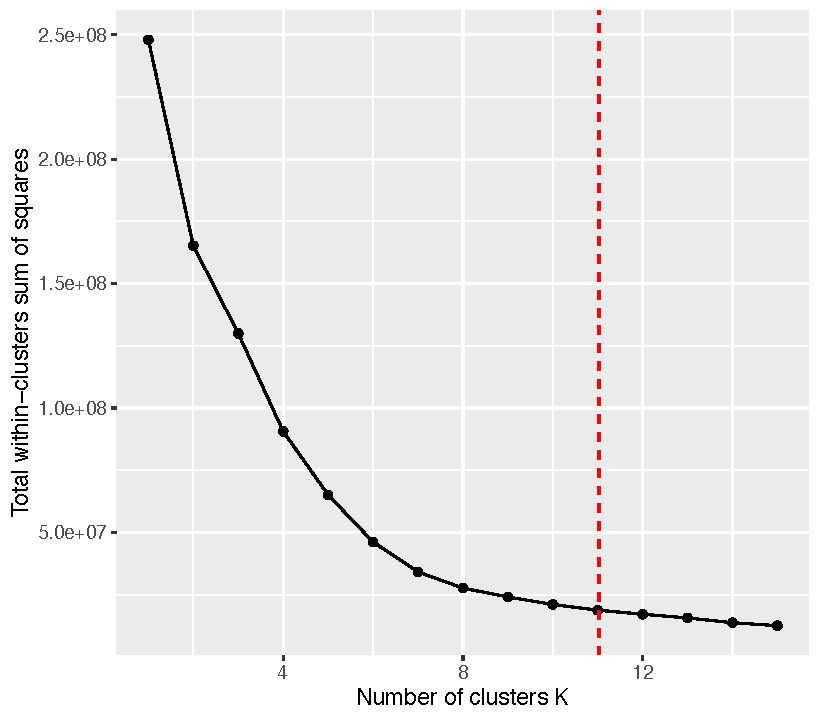
\includegraphics[width=0.4\textwidth]{elbowm.pdf}
\end{center}
\caption{Elbow plot for determining the number of clusters in $K$-means.}\label{figure:elbow}
\end{figure}

\bibliography{tensor_wang}
\bibliographystyle{icml2020}


\end{document}


% This document was modified from the file originally made available by
% Pat Langley and Andrea Danyluk for ICML-2K. This version was created
% by Iain Murray in 2018, and modified by Alexandre Bouchard in
% 2019 and 2020. Previous contributors include Dan Roy, Lise Getoor and Tobias
% Scheffer, which was slightly modified from the 2010 version by
% Thorsten Joachims & Johannes Fuernkranz, slightly modified from the
% 2009 version by Kiri Wagstaff and Sam Roweis's 2008 version, which is
% slightly modified from Prasad Tadepalli's 2007 version which is a
% lightly changed version of the previous year's version by Andrew
% Moore, which was in turn edited from those of Kristian Kersting and
% Codrina Lauth. Alex Smola contributed to the algorithmic style files.
